\subsection{CPU}
\label{sec:cpu}

The computer architecture for the CPU is mainly based on the MIPS architecture. A visual display of the design is shown in figure \ref{fig:ComArch}.

\begin{figure}[H]
    \centering
    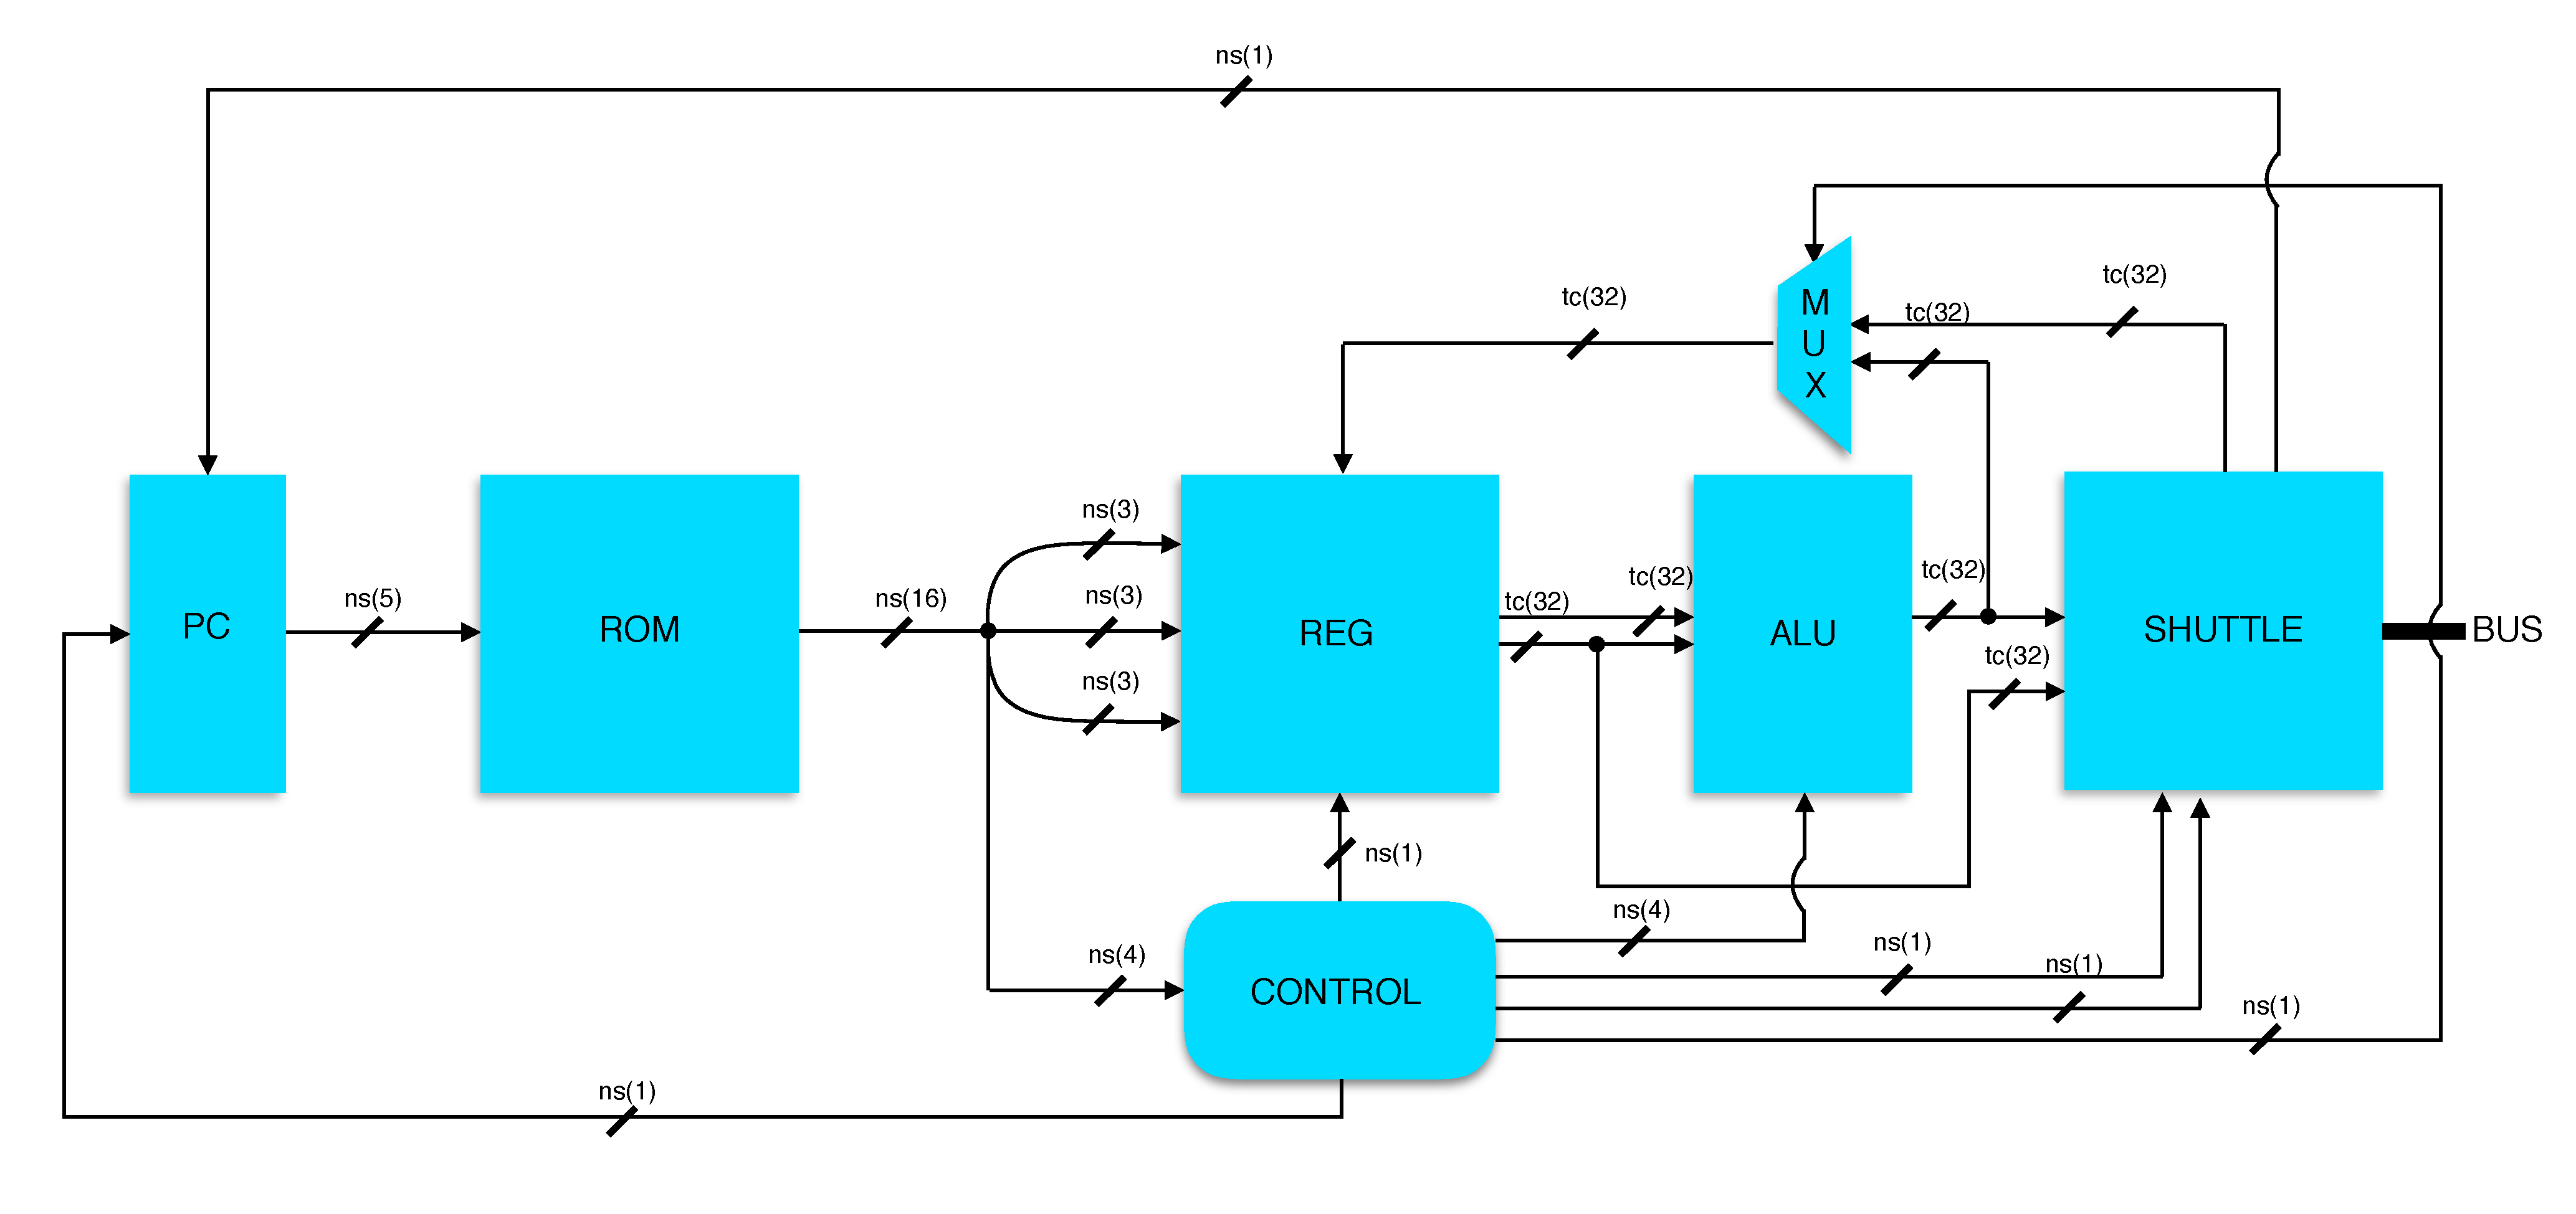
\includegraphics[width=\textwidth]{2Implementation/fig/ComputerArchitecture.pdf}
    \caption{Computer architecture for the CPU. Appendix \ref{app:ComArch} has a large print-friendly version.}
    \label{fig:ComArch}
\end{figure}

The \texttt{PC} contains a register keeping track of the current program counter value. Inside the \texttt{PC} component exists an incrementer and a branching option controlled by the \texttt{CONTROL} component depending on the OPcode (operation code) from the instruction. \\

All instructions are kept in the \texttt{ROM} component. \texttt{ROM} receives an address (the \texttt{PC} value), and sends out the corresponding instruction\footnote{The instruction set is displayed in table \ref{table:InstructionSet}, and the specific program instructions are displayed in table \ref{table:ProgInstructionSet}}. This 16 bit instruction is split into pieces. The pieces are sent to appropriate components. The leading 4 bits are sent to the \texttt{CONTROL}. These 4 bits are the OPcode for the instruction. \\

%After receiving the OPcode, \texttt{CONTROL} determines what computation the CPU does. 
After receiving the OPcode, \texttt{CONTROL} determines which computation the \texttt{ALU} should perform. This is controlled by the use of flags (one bit values, used as booleans). The signal to the \texttt{ALU} is 4 bits long, so the OPcode can be used directly. \\

The \texttt{REG} component contains 8 registers keeping track of all values used for computations, and addresses in external memory.
%and addresses to load and save from/to memory. 
\texttt{REG} receives three parts of the instruction from \texttt{ROM}; AD1, AD2 and AD3 from table \ref{table:InstructionSet}, controlling which registers to read from, and save to. \\
% and to store the new value in. \\

From \texttt{REG}, values from registers AD1 and AD2 are sent to the \texttt{ALU} component. The \texttt{ALU} takes two values and a signal from \texttt{CONTROL}. With these, the \texttt{ALU} performs the desired computation, and sends the result to a \texttt{MUX}, and to the \texttt{SHUTTLE}. This result has two different purposes, depending on the instruction: It is either a value to be stored in a register, or an address in external memory that a value should be saved to, or loaded from. \\

The \texttt{SHUTTLE} component handles communication data flow the to and from the \texttt{BUS} 
% has the main function of talking with the \texttt{BUS},
connecting the CPU to the external memory (RAM). In order to keep communication with the \texttt{BUS} as simple as possible, the \texttt{BUS} is not altered from the template. Everything is controlled in the \texttt{SHUTTLE} inside the CPU instead. \\
\\
The \texttt{SHUTTLE} receives the address from \texttt{ALU} and a value directly from AD2 from \texttt{REG} to store, and two flags from \texttt{CONTROL}. The flags received tells the \texttt{SHUTTLE} whether or not it should send the \texttt{BUS} to memory or not, and if the goal is to load a value from memory or save a value to memory, i.e. specifying the type request. \\
\\
Inside the \texttt{SHUTTLE} is a \texttt{stall} signal checking if the \texttt{BUS} is currently sent to memory. If this is true, the CPU is set to stall. When stalling, the \texttt{PC} does not increment, and the CPU waits for the value from the \texttt{BUS} to reach the \texttt{SHUTTLE}, and get sent to the \texttt{MUX}. \\

For each computation, the \texttt{MUX} component must choose which value to send to \texttt{REG}. This is controlled by a flag from \texttt{CONTROL}. If the instruction requests a value from memory, the \texttt{MUX} forwards the value from \texttt{SHUTTLE}. Otherwise the value from \texttt{ALU} is forwarded.\footnote{In case of a NOP statement, the \texttt{SHUTTLE} value is forwarded through \texttt{MUX}. But the flag from \texttt{CONTROL} tells \texttt{REG} to ignore the input, so no value is stored. Also the AD3 would be 0b000 pointing at register 0, which can not receive a new value.}